\chapter{Synthesizing Data for Object Detection on \ac{MAV}}
\label{sec:training}

Deep learning based Computer Vision models benefit from large training sets which are particularly hard to obtain for \ac{EWFO} detection on \acp{MAV}. Hence, this chapter addresses the generation of data for this application. 

The relevant question to be investigated in this chapter is the following:

\textbf{How can data be generated to train a detection model for \ac{EWFO} detection on a \acp{MAV}?} 

This main question is split in multiple sub questions:
\begin{enumerate}
	\item[\textbf{RQ1.1}] What are the implications of the shape of \acp{EWFO} when synthesizing training data for their detection?
	\item[\textbf{RQ1.2}] How do domain shifts between training and test data affect the detection performance?
\end{enumerate}

In order to investigate these research questions 

This chapter focuses on data generation while the exact model is described in \Cref{sec:object_detection}.







\section{Related Work}
\label{sec:training:related}

Related methods vary from changing low level properties of the image over using CAD models in combination with real background up to rendering full 3D-environments. Often various combinations of synthesized and real data are applied. 

\subsection{Low-Level Image Augmentation}

A common part of current Computer Vision pipelines is to augment a given data set by transforming low level properties of the image. By artificially increasing variations in the input signal, a model that is more invariant to the augmented properties shall be obtained.

\citeauthor{Krizhevsky2012a} \cite{Krizhevsky2012a} use \ac{PCA} to incorporate colour variations. \citeauthor{Howard2013} \cite{Howard2013} shows how several image transformations can improve the performance of a \ac{CNN}-based Classification model. The proposed pipeline includes variations in the crop of the input image as well as variations in brightness, color and contrast. In \ac{CNN}-based Object Detection \citeauthor{Redmon} \cite{Redmon} uses random scaling and translation of the input image, as well as random variations in saturation and exposure. \citeauthor{Liu} \cite{Liu} additionally crop and flip each image with a certain probability.

Since most methods use image augmentation and \citeauthor{Krizhevsky2012a} \cite{Krizhevsky2012a} mentions it to be the particularly reason for superior performance at ILSVRC2012 competition it can be assumed to be beneficial for Computer Vision models. Unfortunately, none of the publications measures the improvements gained by the different operations. 

While the aforementioned approaches add artificial variation to the input data, \citeauthor{Carlson2018}\cite{Carlson2018} augment the image based on a physical camera model. The proposed pipeline is applied for Object Detection and incorporates models for sensor and lens effects like chromatic aberration, blur, exposure and noise. While being of minor effect for the augmentation of real data (0.1\% - 1.62\% \ac{mAP}70) the reported results show an improvement when training on fully synthesized datasets. Here the reported gains vary between 1.26 and 6.5 \% \ac{mAP}70.

Low-level image augmentation is a comparatively cheap method to increase the variance in a dataset. However, it cannot create totally new samples or view points. Furthermore, it cannot change the scene in which an object is placed. Therefore it needs a sufficiently large base dataset that is augmented. This work addresses the case when no real training data is available. Hence, low-level image augmentation is incorporated in the training process but can not be the only method applied.

\subsection{Augmenting Existing Images with CAD - Models}

In order to create new view points \ac{CAD}-models can be used. These models describe 3D-shape of an object and can be placed on existing images to augment or increase a dataset.

\citeauthor{Peng}\cite{Peng} study the use of \ac{CAD}-models in the context of \ac{CNN}-based Object Detection. The authors particularly address how image cues like texture, colour and background affects the detection performance. The experiments show how the used \acp{CNN} are relatively insensitive towards context but use shape as primary, texture and colour as secondary most important features. This enables competitive performance even when the object of interest is placed only on uniformly covered backgrounds. However, the study only covers solid objects such as birds, bicycles and airplanes. \ac{EWFO} are substantially different and we hypothesize that other image cues must be relevant.

\citeauthor{Madaan2017}\cite{Madaan2017} study the segmentation of wires based on synthetic training. As wires similarly to \ac{EWFO} only consist of thin edges, the application is quite close to this work. However, the experiments focus on a single domain, namely sky images and thus the variations in background are comparatively small. We hypothesize that \ac{EWFO} are particularly sensitive to such variations and address the application in multiple domains.

\citeauthor{Hinterstoisser2017} \cite{Hinterstoisser2017} propose to use a base network that has been trained on real images and to continue training on images with \ac{CAD}-models. During training the base network is frozen and only the last layers are updated. The method does not use real data but requires a suitable base network. As most available feature extractors (further discussed in \Cref{sec:object_detection}) are of a size that is computationally prohibitive for \ac{MAV} the method is not really applicable for this work. 

The use of CAD-models in combination with real backgrounds allows to generate totally new view points for the object of interest. Furthermore, the image background consists of real data and thus the synthetic textures only concern the rendered object. However, the geometric properties like perspective as well as the physical properties like object placement are violated and therefore create an artificial scene. Despite this fact, literature shows that such images can benefit model performance in various cases. Yet, most of the approaches still use real data and/or focus on solid objects with rich textures and complex shape. We hypothesize that since \ac{EWFO} do not provide these kind of structures the results do not apply in the same way. Hence, we incorporate the method to generate data and investigate how it can be applied for the detection of \ac{EWFO}.

\subsection{Fully Synthesizing Environments}

A more realistic placement of objects can be achieved when fully synthesizing environments.  The object of interest can be placed according to physical laws, shadows fall correctly and geometric properties of an image are followed. However, if the graphical models do not fully capture the details of real world objects, the generated data might look too artificial.

\citeauthor{Johnson-Roberson2016} \cite{Johnson-Roberson2016} use a powerful graphical engine and a highly detailed environment to train an Object Detection model entirely in simulation. The results show an improvement towards data annotated by humans especially when using vast amounts of simulated data. \todo{There should be more examples for this} 

In order to create realistic environments intense manual work is required for the design. In contrast \cite{Sadeghi2016, Tobin2017, Tremblay2018a} use a relatively simple environment but a high degree of randomization to address the reality gap. The aim is to learn an abstract representation by strongly varying textures, light conditions and object locations. \citeauthor{Tobin2017} introduced this technique as \ac{DR}. The drawback of the approach is that a too high degree of randomization may omit pattern in the target domain that could otherwise be exploited by the model. 

This work addresses the generation of data for the detection of \ac{EWFO} on \acp{MAV} in \ac{GPS} denied scenarios. Such scenarios cover a wide range of possible environmental conditions and the images taken from \ac{MAV} cameras are peculiar. Hence the creation of a full environment is investigated in this work. 


\subsection{Transfer Learning}

The field of transfer learning particularly addresses domain shifts in the modelling process. Hence, a common application is the learning from synthetic data.

A common approach in \ac{CNN}-based models is the incorporation of a domain classifier in the model. By augmenting the data with domain labels, the classifier learns to distinguish the two domains. Subsequently a gradient reverse layer is applied and thus the weights are updated in such a way that a domain agnostic representation is learned. Examples of the approach can be found in \cite{Chen2018c} \cite{Xu2017}.

While the aforementioned approaches require labelled samples from the target domain, \citeauthor{Peng2017} \cite{Peng2017} propose to include task-irrelevant samples and a source classifier. As a result no samples of the target domain are required.

While transfer learning provides the theoretical framework as well as methods to deal with domain shifts, it does not allow to generate data. Furthermore, it often requires samples of the target domain. This work addresses the case when no real data is used for training. The field is interesting to be incorporated in the data generation pipeline investigated in this thesis but it can not be used as a start off point. Hence, the use of transfer learning in the modelling process is denoted as future work.

\subsection{Generative Adversarial Networks}

\cite{Inoue} 
\todo{write}

\section{Methodology}

In order to to investigate the research questions a data generation pipeline is implemented using OpenGL, UnrealEngine and AirSim. An overview can be seen in \Cref{fig:training:datagen_notation}. In the first step a scene is created in which the objects of interest as well as the camera are placed. In 3D space position and orientation (pose) of each object are determined by translation $\textbf{t}$ and rotation $\textbf{r}$. The coordinate system is \ac{NED}.

A view projection yields an image through the lens of the camera. The coordinates of each point in 3D space are projected on the 2D image plane. A final post processing step can simulate further effects like lens distortion and sensor noise. This step is implemented using OpenCV and Python.

\begin{figure}[htbp]
	\centering
	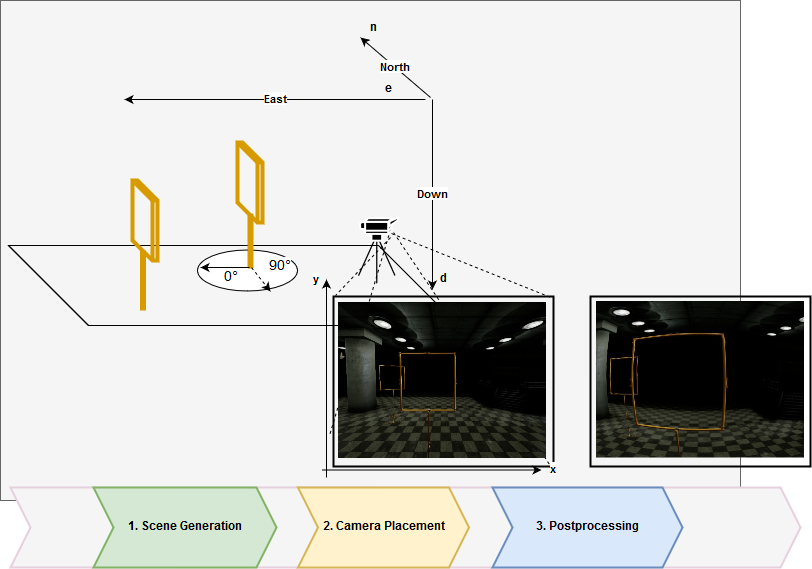
\includegraphics[width=\textwidth]{fig/datagen_notation}
	\caption{Overview of the data generation process.}
	\label{fig:training:datagen_notation}
\end{figure}



\subsection{Generating a Scene}
\label{sec:training:scene}

The first step determines the environment in which the object is embedded. This contains context such as background and other objects, as well as light conditions. 

The experiments in \cite{Peng} show how \acp{CNN} are relatively independent from these kind of image cues. Even trained on uniformly coloured backgrounds an object detector is able to achieve competitive performance. Instead \acp{CNN} seem to exploit texture and shape of the object. However, the objects investigated are solid which is not the case for \ac{EWFO}. \ac{EWFO} have a distinctive shape but the main part of their surface contains background. We hypothesize this makes the detection of the shape harder. Furthermore, \ac{EWFO} do not provide texture that can be exploited by a detector, which further complicates the detection. We hypothesize that \ac{EWFO} are more dependent on background than solid texture rich objects. 

Placing a \ac{CAD}-model on existing images allows to generate samples without fully synthesizing an environment. In literature \cite{Madaan2017, Peng} approaches can be found that show the success of this method. However, without a realistic environment geometric properties of real images are violated. Furthermore, light conditions do not align with the rest of the scene. Hence, we hypothesize that only placing a \ac{CAD}-model on existing images leads to a too artificial learning setting. An object detector trained in such an environment might learn only to predict the object that does not fit to the rest of the scene.

In order to evaluate the hypotheses several training and test environments are created. A black environment serves as base to replace the background with existing images. Furthermore, three indoor base environments are created that fully simulate illumination and background. An overview can be seen in \Cref{fig:environments}. Within the environment light conditions, background textures, object locations can be changed manually. The environments are described in the following:

\begin{enumerate}
	\item \textit{Dark:} The environment is a room without windows, only containing artificial light sources. 
	\item \textit{Daylight:} The environment is a room with windows along all walls that allow daylight to illuminate the room. The windows can lead to strong variations in the contrast between different parts of the object.
	\item \textit{IROS:} The environment resembles the room of the \ac{IROS} Autonomous Drone Race 2018. The light sources stem from a window front at one side of the room, as well as artificial light sources at the ceiling. Depending on the view point, the object might appear against bright or dark background.
\end{enumerate}

\begin{figure}[hbtp]
	\centering
	\begin{minipage}{0.3\textwidth}
		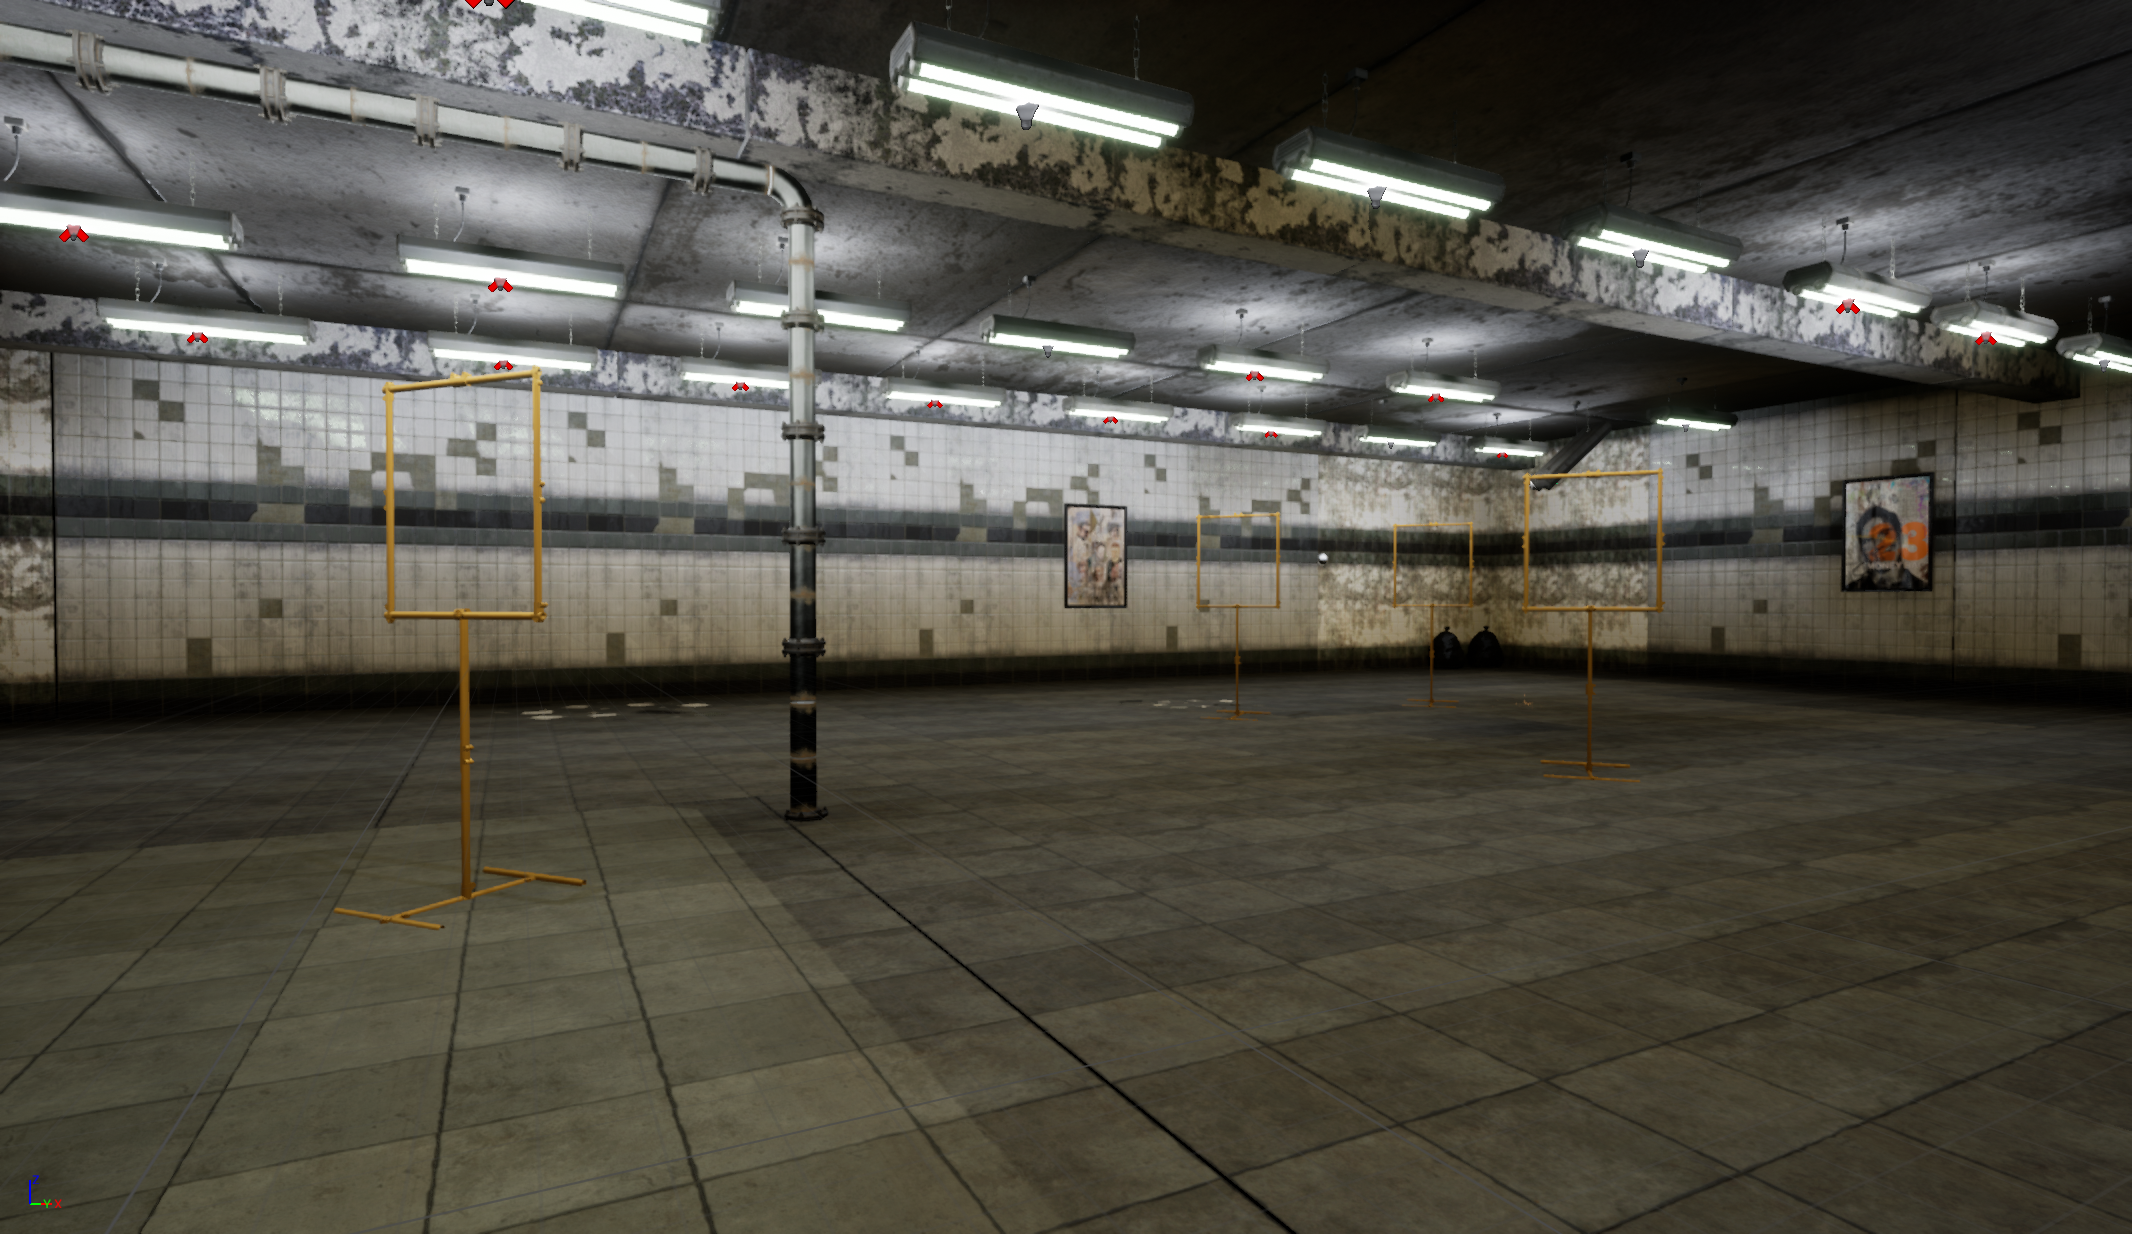
\includegraphics[width=\textwidth]{fig/basement_perspective}
	\end{minipage}
	\begin{minipage}{0.3\textwidth}
		\includegraphics[width=\textwidth]{fig/daylight_perspective}
	\end{minipage}
	\begin{minipage}{0.3\textwidth}
		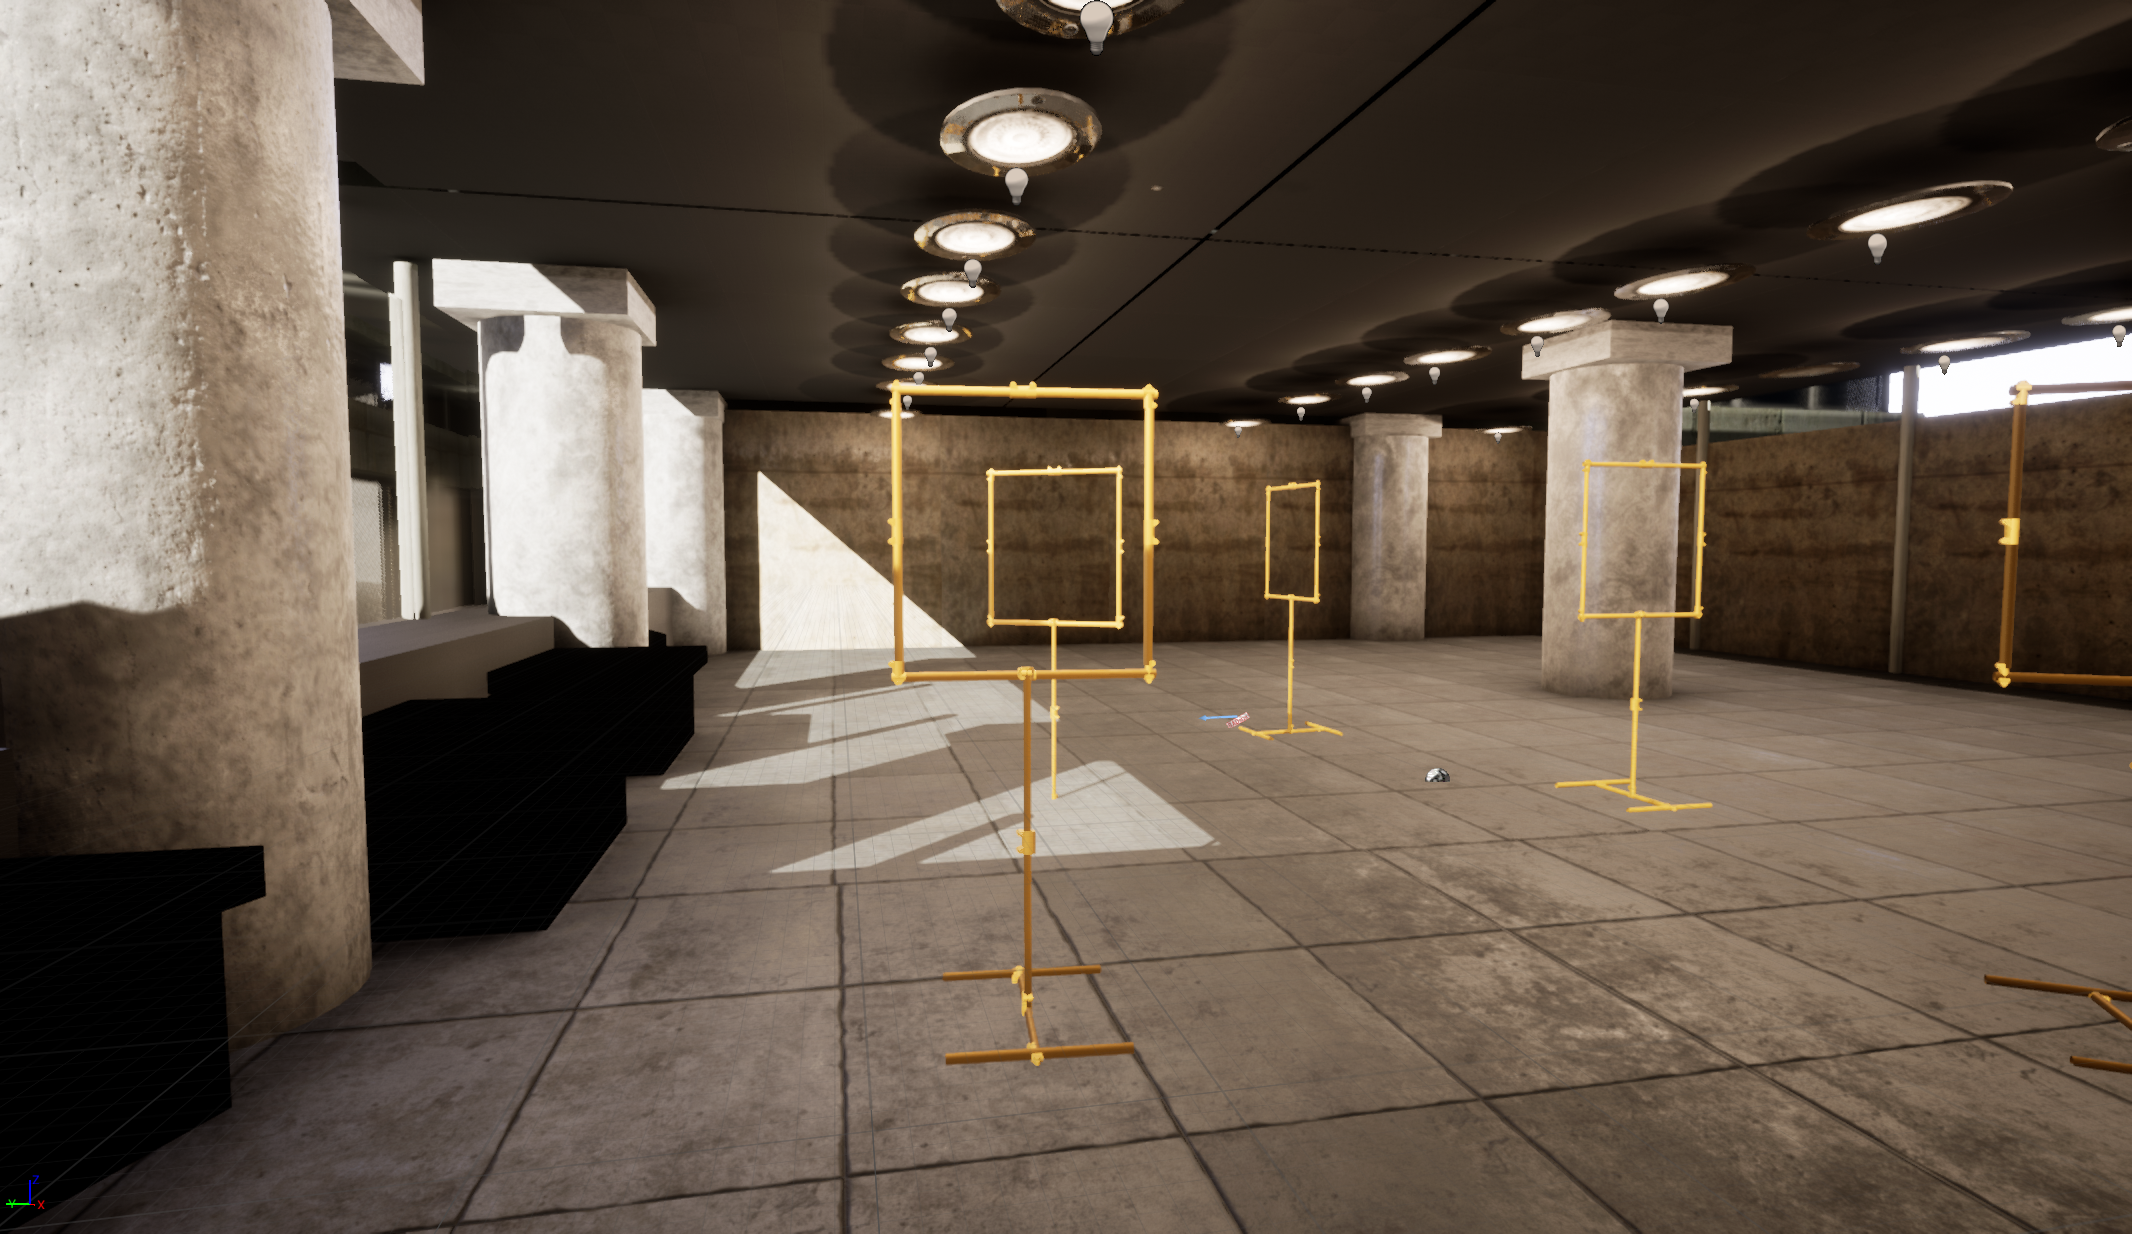
\includegraphics[width=\textwidth]{fig/iros_perspective}
	\end{minipage}
	\caption{\textit{IROS2018} Environment.}
	\label{fig:environments}
\end{figure}


\subsection{Placing the Camera}

Another important property that influences the generated sample is the camera pose. It determines the view on the scene and therefore at which distance, angle and location the objects appear on the image.

A straightforward way is placing the camera at random locations within the scene \todo{double check}. However, such a placement might not resemble the real world sufficiently. An \ac{MAV} does not appear at random places within a scene, especially not when it follows a racing track. \acp{CNN} are translation invariant by design but cannot inherently handle variation in rotation and scale. We hypothesize that placing the camera does not cover sufficient views on the object of interest. 

In order to evaluate our hypothesis, we incorporate the pattern of following a race track with an \ac{MAV} in the data generation process. A motion model of a quad-rotor \ac{MAV} is implemented and a velocity controller is used to make the camera follow a certain trajectory in the environment. The environment is set up in way that it resembles a race court.  Storing the current image at a frequency of 2 Hz creates the corresponding samples. The development of this model has not been done within this thesis but is summarized here for completeness: \todo{put shuos model here}. 

When following the race track, the camera focuses the next object frontally most of the time. The appearance of the object increases as the camera approaches until the gate has been passed. This is also resembled when looking at the bounding box locations and dimensions.

\begin{figure}
	\begin{minipage}{\textwidth}
		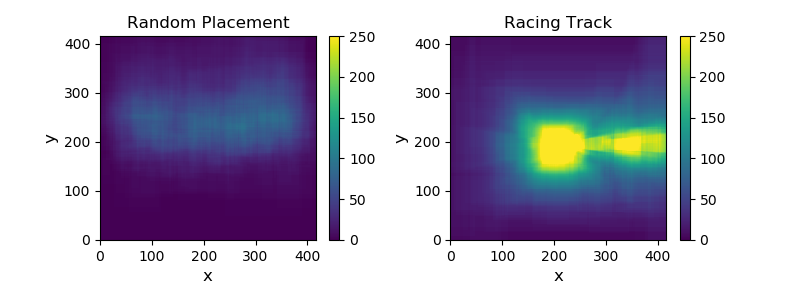
\includegraphics[width=\textwidth]{fig/heatmap_camplace}
		\caption{Heatmaps based on bounding boxes. Left the distribution when using random placement, right when moving through the scene with a drone motion model.}
		\label{fig:heatmap_camplace}
	\end{minipage}
	\begin{minipage}{\textwidth}
		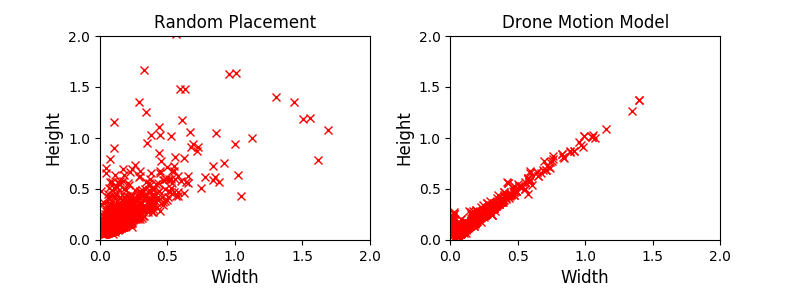
\includegraphics[width=\textwidth]{fig/aspect_ratios_camplace}
		\caption{Scatterplot of bounding box dimensions.}
		\label{fig:scatter_camplace}
	\end{minipage}
\end{figure}

\Cref{fig:heatmap_camplace} shows the distribution of bounding boxes when created with the two methods. It can be seen how with the drone motion model most of the objects are centered and distributed across the horizon. In contrast, the random placement leads to more evenly distributed object locations.\todo{replace this with clusters by angle and distance}

\Cref{fig:scatter_camplace} shows a scatterplot of the bounding box dimensions. With the drone motion model one can see how the bounding box aspect ratio is mostly close to one, which appears when the object is faced frontally. The dimensions are increasing linearly as the camera approaches the object. The random placement on the other hand creates a larger variance in bounding box dimensions. This is due to the fact that more relative views towards the object are created. 

\Cref{fig:scatter_camplace} also shows how the dataset generated with random placement does not contain many objects with an aspect ratio close to 1. Hence, samples where the object appears , faced frontally with low distance do almost not appear in this generated set. With the drone motion model on the other hand several such samples exist.

We hypothesize that the generation of samples with only one of the two methods misses important object appearances. Random placement does not cover most common appearances such as when flying through the racing gate. The drone motion model tends to limit object appearances depending on the flown trajectory as well as the created race court.


\subsection{Post-processing}

After having created a set of 2D images, the final step applies low-level image transformations. It allows to further simulate sensor effects and increase the variance in the generated data.

In literature \cite{Krizhevsky2012a,Howard2013,Redmon,Liu} the application of image augmentation is a common tool to improve the detection performance. The experiments in \cite{Carlson2018} show how the incorporation of sensor effects particularly improves the performance of models learned on fully synthesized data. In the \ac{MAV} domain sensor and lens effects have a significant influence on the obtained sample. Hence, we hypothesize that the incorporation of these effects is particularly useful for the \ac{MAV} domain.

\paragraph{Lens Distortion}

Lens distortion is a form of optical aberration which causes light to not fall in a single point but a region of space. For \acp{MAV} commonly used wide-angle lenses, this leads to barrel distortion and thus to straight lines appearing as curves in the image.

The effect is applied using the model for wide-angle lenses from \cite{Vass}. It models the removal of lens distortion as combination of radial and non-radial part, that is approximated with a second order Taylor expansion:
\todo{double check formula is (y in first line?)}
\begin{equation}
f(x,y) =
\begin{pmatrix}
x (1 + \kappa_1 x^2 + \kappa_1 (1 + \lambda_x) y^2 + \kappa_2(x^2 + y^2)^2) \\
y (1 + \kappa_1 x^2 + \kappa_1 (1 + \lambda_y) y^2 + \kappa_2(x^2 + y^2)^2)
\end{pmatrix} 
\label{eq:distortion}
\end{equation}
Where:
\begin{itemize}
	\item f yields the undistorted coordinates.
	\item $\kappa_1$ $\kappa_2$ control the radial distortion 
	\item $\lambda_x$ and $\lambda_y$ control the tangential distortion
\end{itemize}
 
Applying the lens distortion to an image is done using the inverse of \Cref{eq:distortion}. However, as there is no closed form solution, so the Newton-approximation.

An example with $\kappa_1 = 0.5, \kappa_2 = 0.5$ is displayed in \Cref{fig:distortion}. It can be seen how the previously straight lines appear as circular shape.

\paragraph{Chromatic Aberration.}

Chromatic Aberration is caused when different wavelengths of light do not end up in the same locations of the visual sensor. This leads to a shift in the colour channels of the image.

Similarly to \cite{Carlson2018}, chromatic aberration is applied by scaling the locations of the green channel, as well as applying translations on all channels. The model can be implemented as affine transformation of the pixel locations for each channel:

\begin{equation}
f(x_C,y_C) = \begin{pmatrix}
S & 0 & t_x \\
0 & S & t_y \\
0 & 0 & 1
\end{pmatrix} \begin{pmatrix}
x_C \\
y_C \\
1
\end{pmatrix}
\end{equation}

Where $C$ is one colour channel of the image.

An example is displayed in \Cref{fig:chromatic}. It can be seen how the red and green channel are shifted relative to each other. Thus two bars appear in the image.

\paragraph{Blur}

Motion noise is caused when light falls in different locations of the images sensor due to a fast movement of the camera. It leads to blurry images based on the sensor motion.

The phenomenon depends on camera properties as well as the motion of camera and objects. Although a full modelling of this process might benefit the learning process, it requires a complex pipeline and is computationally expensive. Therefore a strong simplification is used, namely a one-dimensional Gaussian filter:

An example for vertical blur is displayed in \Cref{fig:motionblur}. It can be seen how particularly horizontal lines appear softer.

Next to motion, sensor noise can lead to blurry images. For the blur operation a 2D Gaussian kernel is applied on the input image with:

\begin{equation}
 k = \frac{1}{2\sigma_x\sigma_y\pi}e^{-\sqrt{\frac{x^2 + y^2}{2\sigma_x\sigma_y}}} 
\end{equation}
\todo{double check notation}
\paragraph{Exposure.}

Exposure is the time the sensor records light in order to create an image. Over- and Underexposure are caused when this time is too short or too long, leading to too dark or too bright images.

Following the model from \cite{Carlson2018}:
 
\begin{equation}
f(S) = \frac{255}{1 + e^{-A S}}
\end{equation}
where $A$ is a constant term for contrast and $S$ the exposure.
\todo{whats a}
The image can be re-exposed with:

\begin{equation}
	I' = f(S+\Delta S)
\end{equation}

where $S$ is obtained from :
\begin{equation}
S = f^{-1}(I)
\end{equation}

An example for overexposure is displayed in \Cref{fig:exposure}. It can be seen how lighter areas appear particularly light, while dark areas remain dark.

\subsection{Color Variations}

\todo{describe hsv scaling}


\begin{figure}[htbp]
	\centering
	\begin{minipage}{0.33\textwidth}
		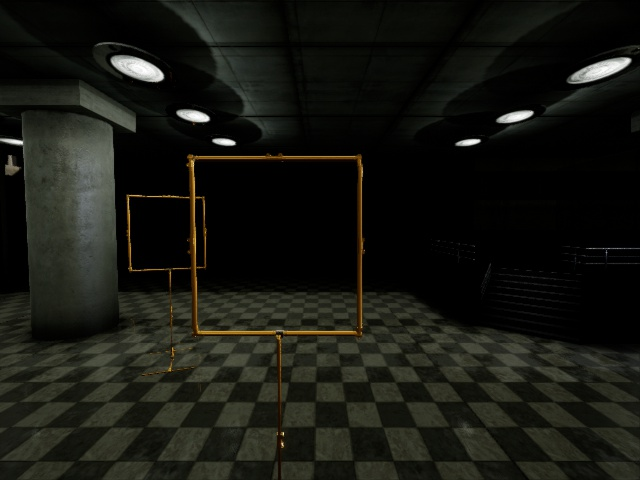
\includegraphics[width=\textwidth]{fig/gate_example}
\caption{Original Image.}
\label{fig:orig}
	\end{minipage}
	\begin{minipage}{0.33\textwidth}
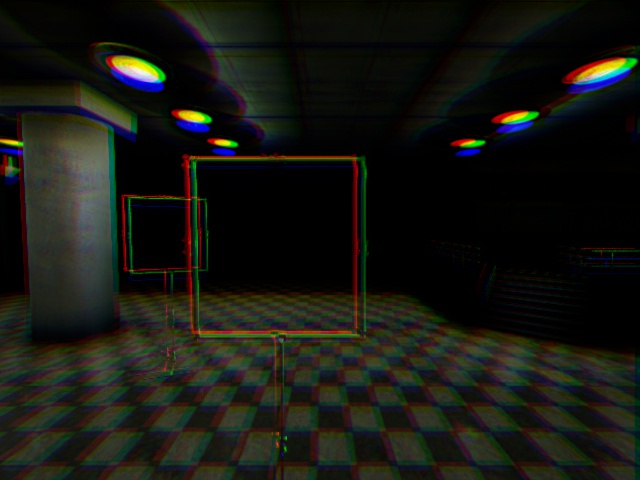
\includegraphics[width=\textwidth]{fig/gate_example_chromatic}
	\caption{Chromatic Aberration.} 		
	\label{fig:chromatic}
\end{minipage}
	\begin{minipage}{0.33\textwidth}
		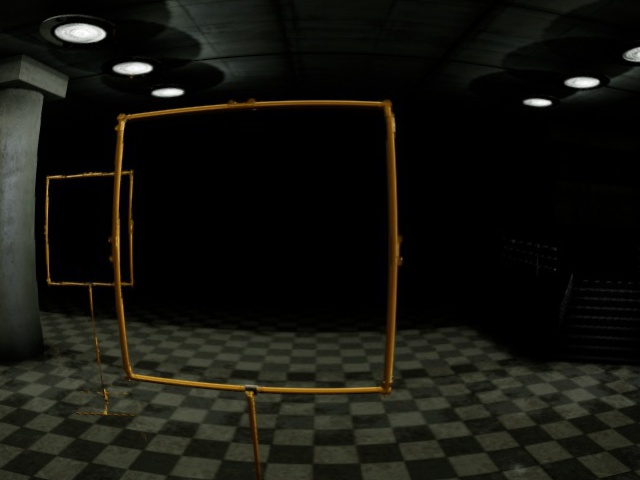
\includegraphics[width=\textwidth]{fig/gate_example_distorted}
	\caption{Lens Distortion. }		
\label{fig:distortion}
	\end{minipage}

	\begin{minipage}{0.33\textwidth}
		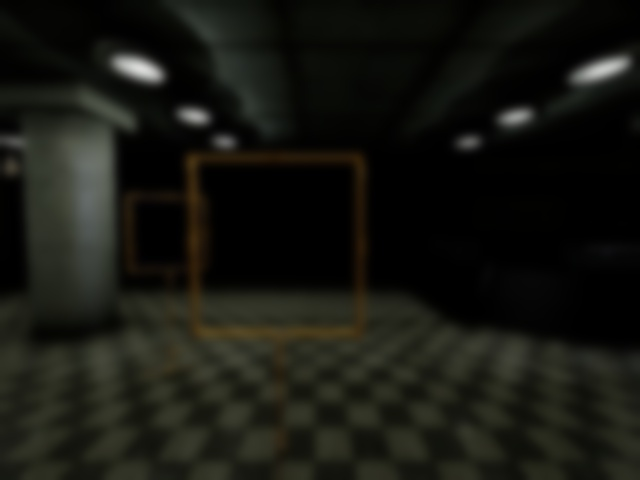
\includegraphics[width=\textwidth]{fig/gate_example_focusblur}
	\caption{Out-of-Focus blur.}
\label{fig:focusblur}
	\end{minipage}
	\begin{minipage}{0.33\textwidth}
		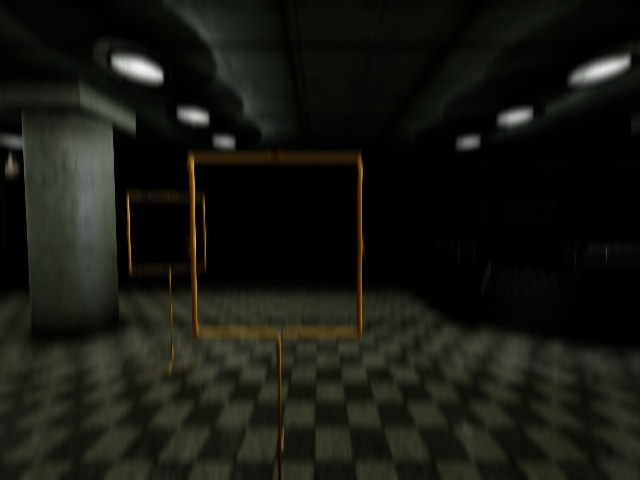
\includegraphics[width=\textwidth]{fig/gate_example_motionblur_v}
	\caption{Vertical Motion Blur.}
\label{fig:motionblur}
	\end{minipage}
	\begin{minipage}{0.33\textwidth}
		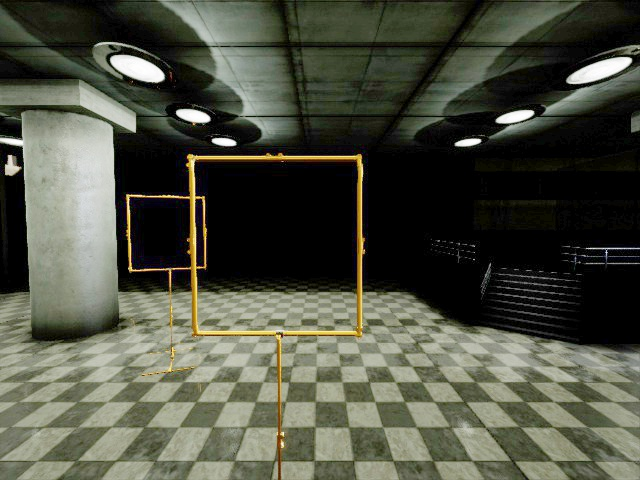
\includegraphics[width=\textwidth]{fig/gate_example_exposure}
	\caption{Exposure.}
\label{fig:exposure}
	\end{minipage}
\end{figure}

\subsection{Hypothesis}
\label{sec:training:hypothesis}

This chapter summarizes the hypotheses formulated in the previous chapters:

\begin{enumerate}
	\item[$\mathcal{H}_1$] An object that is not empty and provides a more distinctive structure is less background dependent than an \ac{EWFO}.
	
	\item[$\mathcal{H}_2$] The incorporation of correct placement/light conditions improves the performance of a model trained to detect \acp{EWFO}.
	
	\item[$\mathcal{H}_3$] The incorporation of a camera motion model resembling the target domain improves the performance of a model trained to detect \acp{EWFO}. 
	
	\item[$\mathcal{H}_3$] Including sensor effects present in the target domain, improves the performance of a model trained to detect \acp{EWFO}. 
	
\end{enumerate}



\section{Experiments}
\label{sec:training:experiments}
In order to evaluate the formulated hypotheses several experiments are conducted. The model used is the TinyYoloV3-Architecture, further described in \Cref{sec:object_detection}. The reported metrics are described in \Cref{sec:metrics}. For all experiments mean and standard deviation of 5 runs are reported.

For the random view point generation the following parameters are used:

\begin{equation}
	x = \mathcal{U}(-30,30),\quad y = \mathcal{U}(-20,20),\quad z = \mathcal{N}(-4.5,0.5)),\quad
	\phi = \mathcal{U}(0,0.1\pi),\quad \theta = \mathcal{U}(0,0.1\pi),\quad \psi = \mathcal{N}(-\pi,\pi)
	\label{eq:distroexp}
\end{equation}
Where $ \mathcal{U}(a,b)$ is a uniform distribution between $a,b$ and $\mathcal{N}(\mu,\sigma^2)$ is a Gaussian distribution with mean $\mu$ and variance $\sigma^2$.

The parameters are chosen experimentally aiming to resemble common view points of a person standing in the room.

\subsubsection{Experiment I}
The empty space of an \ac{EWFO} is augmented with a texture rich structure. An example can be seen in \todo{text}. The object is placed in a scene with uniformly colored backgrounds and a training set of 20 000 samples is created. In similar fashion a training set is created without the texture rich augmentation. On both objects an object detector is trained and subsequently evaluted in a test set. The test set contains 1000 samples created by placing objects in a fully synthesized environment.

\subsubsection{Experiment II}

Several models are trained on 20 000 samples each.
\begin{itemize}
	\item[ModelU] Uniform
	\item[ModelSVE] Single Virtual Environment
	\item[ModelRB] Real Backgrounds
	\item[ModelVVE] Various Virtual Environments
	\item[ModelRBVVE] Real Backgrounds + Various Virtual Environments
\end{itemize}


\begin{table}[htbp]
	\caption{}
	\begin{tabular}{|l|l|l|l|r|r|r|l|l|l|}
		\hline
		& Validation Set &  &  & \multicolumn{1}{l|}{IROS2018} & \multicolumn{1}{l|}{} & \multicolumn{1}{l|}{} & Real Data &  &  \\ \hline
		& AP40 & AP60 & AP80 & \multicolumn{1}{l|}{AP40} & \multicolumn{1}{l|}{AP60} & \multicolumn{1}{l|}{AP80} & AP40 & AP60 & AP80 \\ \hline
		U &  &  &  & 0.05 & 0.01 & 0 &  &  &  \\ \hline
		SVE &  &  &  & 0.29 & 0.17 & 0.02 &  &  &  \\ \hline
		VVE &  &  &  & 0.61 & 0.49 & 0.17 &  &  &  \\ \hline
		RB &  &  &  & 0.42 & 0.28 & 0.04 &  &  &  \\ \hline
	\end{tabular}
	\label{tab:env}
\end{table}


\subsubsection{Experiment III}

Three models are trained: Model I using random placement, Model II using the drone motion model, Model III using a combination of both methods. In both experiments environment and light conditions as well as object locations are the same. The models are tested on two test sets: Set I created by randomly placing the camera. Set II by using the drone motion model, where a circuit is used that has not been part in the generation of the training data.


\subsubsection{Experiment IV}

In order to evaluate $\mathcal{H}_4$ the individual domain properties are measured on the target domain and incorporated in the training set.


\section{Results}
\label{sec:training:results}

\section{Discussion}
\label{sec:training:discussion}

\section{Conclusion}
\label{sec:training:conclusion}


